% Chapter 2: The breadth-first walk
% Contains:
%   The definition of the breadth-first walk
%   The continuous version
%   The proof of Zn -> W

\chapter{The breadth-first walk}
\fxnote{Update title.}


\section{The discrete breadth-first walk}
%%%%%%%%%%%%%%%%%%%%%%%%%%%%%%%%%%%%%%%%%%%%%%%%%%%%%%%%%%%%
% SECTION: The discrete breadth-first walk
%%%%%%%%%%%%%%%%%%%%%%%%%%%%%%%%%%%%%%%%%%%%%%%%%%%%%%%%%%%%
\fxnote{Update title}

%%%%%%%%%%%%%%%%%%%%%%%%%%%%%%%%%%%%%%%%%%%%%%%%%%%%%%%%%%%%
% Introduction
%%%%%%%%%%%%%%%%%%%%%%%%%%%%%%%%%%%%%%%%%%%%%%%%%%%%%%%%%%%%
We start by describing the deterministic construction of the breadth-first walk.
\fxnote{More free from paper}
Consider an arbitrary graph $\mathcal{G}$ on the set of vertices 
$\{1, \dots , n\} $.
We will define the breadth-first ordering
$(v(1), \dots v(n))$
of the vertices along with an integer-valued sequence
$(z(i), \; 1 \leq i \leq n)$
which we call the breadth-first walk on
$\mathcal{G}$.


%%%%%%%%%%%%%%%%%%%%%%%%%%%%%%%%%%%%%%%%%%%%%%%%%%%%%%%%%%%%
% Definition of breadth-first order
%%%%%%%%%%%%%%%%%%%%%%%%%%%%%%%%%%%%%%%%%%%%%%%%%%%%%%%%%%%%
The breadth-first order follow an algorithmic construction as follows:
Let $\Ci{1}, \Ci{2}, \dots$ be the components of $\mathcal{G}$ in order, such that
$w_1, w_2, \dots$, the vertices with the smallest label in the corresponding component,
are ordered $w_1 > w_2 > \dots$. 
Call $w_i$ the root of $\Ci{i}$.
Now order by levels (distance from the root) and within levels order by original vertex label.
See Figure \ref{F: bf-walk} for an example of the new ordering.

For a more mathematically concise definition,
consider the set of vertices $\{ v(1),\dots, v(i) \}$
and define the \emph{neighbour set} $\Ni{i}$ as the vertices outside of
\fxnote{Add emphasis when needed}
$\{ v(1),\dots, v(i) \}$ 
that are neighbours to some vertex in 
$\{ v(1),\dots, v(i) \}$:
\begin{equation}
\Ni{i} := 
\left\lbrace v \in \{1, \dots, n\} \backslash \{ v(1),\dots, v(i) \} 
\; | \; 
\left(v(j), v\right) \in S \; \text{for some} \; 1 \leq j \leq i \right\rbrace
\end{equation}
\fxnote{Remove equation? Unnecessary?}
\fxnote{Fix \text in braces: Space \; or \quad}
This allows us to define the set of children of some vertex $v(i)$ as
$\Ni{i} \backslash \Ni{i-1}$.
First order the components as described above. 
Now consider only the first component $\Ci{1}$.
Define $v(1) := w_1$, the root of $\Ci{1}$ and define
$v(2), \dots , v(1 + |\Ni{1}|)$ 
as the neighbours of $v(1)$,
in increasing order of vertex label. 
Define the new label for all 
$i = 2, \dots, |\Ci{1}|$,
that is all vertices in the first component,
inductively by listing all children (if any exist) of $v(i)$
in increasing order as 
$ v(i + |\Ni{i-1}|), \dots, v(i + |\Ni{i}|) $.
After labeling the last vertex in $\Ci{1}$, set
$v(|\Ci{1}| + 1) := w_2$, 
the root of $\Ci{2}$, and continue the construction as above.
Traverse all components this way.


%%%%%%%%%%%%%%%%%%%%%%%%%%%%%%%%%%%%%%%%%%%%%%%%%%%%%%%%%%%%
% Definitions of breadth-first walk
%%%%%%%%%%%%%%%%%%%%%%%%%%%%%%%%%%%%%%%%%%%%%%%%%%%%%%%%%%%%
For the number of children of $v(i)$ write 
$c(i) = |\Ni{i} \backslash\Ni{i-1}|$.
Now define the breadth-first walk 
$(z(i), \; 1 \leq i \leq n)$
by
\begin{equation} \label{E: def bf-walk z}
\begin{aligned}
z(0) &:= 0, \\
z(i) &:= z(i-1) + c(i) -1, \quad i=1, \dots , n.
\end{aligned}
\end{equation}


%%%%%%%%%%%%%%%%%%%%%%%%%%%%%%%%%%%%%%%%%%%%%%%%%%%%%%%%%%%%
% Explanation
%%%%%%%%%%%%%%%%%%%%%%%%%%%%%%%%%%%%%%%%%%%%%%%%%%%%%%%%%%%%
An explanation:
\fxnote{Change this}
The process divides the vertex-set into three parts: 
Explored, discovered and neutral vertices. Every vertex starts as neutral.
At step $1$, we traverse vertex $v(1)$ and mark it as explored.
We search for neighbours of $v(1)$, and mark these as discovered.
The next vertex to explore is the vertex already discovered with the smallest label,
and each vertex switches from neutral to discovered once it gets assigned a new label.
Once it's neighbours are explored, it switches to explored.
\fxnote{This whole paragraph}
Note that after traversing every vertex of one component, 
there are no discovered vertices left.
The walk $z$ decreases by $1$ for each vertex traversed
and increases by the number of new neighbours explored in each step.


\begin{figure}[H]
	\label{F: bf-walk}
	
	\centering
	\subfloat[Original vertex labels]
	{\begin{tikzpicture}[level distance = 11mm, scale = 1]
	\tikzstyle{level 1}=[sibling distance=8mm]
	\tikzstyle{level 2}=[sibling distance=8mm]
	\tikzstyle{level 3}=[sibling distance=8mm]
	
	\node [plain] (1) {1} [grow=up]
	child { node [plain] {\phantom{0}}
		child { node [plain] {\phantom{0}}
		}
		child { node [plain] {\phantom{0}}
		}
	}
	child { node [plain] {\phantom{0}}
	}
	;
	\node [plain] [right=2.5cm of 1] (6) {2} [grow=up]
	child { node [plain] {\phantom{0}}
		child { node [plain] {6}
		}
		child { node [plain] {\phantom{0}}
		}
		child { node [plain] {\phantom{0}}
		}
	}
	child { node [plain] (8) {\phantom{0}}
	}
	child { node [plain] {\phantom{0}}
		child { node [plain] (10) {\phantom{0}}
		}
	}
	;
	\node [plain] [right=2cm of 6] (14) {3} [grow=up]
	child { node [plain] {\phantom{0}}
	}
	;
	\node [plain] [right=1cm of 14] (16) {4} [grow=up]
	child { node [plain] {\phantom{0}}
	}
	child { node [plain] {\phantom{0}}
	}
	;
	\node [plain] [right=1cm of 16] (19) {5}
	;
	\node [plain] [right=1cm of 19] (20) {7} [grow=up]
	child { node [plain] {\phantom{0}}
	}
	child { node [plain] {\phantom{0}}
		child { node [plain] {\phantom{0}}
			child { node [plain] {\phantom{0}}
			}
			child { node [plain] {\phantom{0}}
			}
			child { node [plain] {\phantom{0}}
			}
			child { node [plain] {\phantom{0}}
			}
		}
	}
	;
	\draw (10) -- (8);
\end{tikzpicture}}\\
	
	\centering
	\subfloat[New vertex labels]
	{\begin{tikzpicture}[level distance = 11mm, scale = 1]
	\tikzstyle{level 1}=[sibling distance=8mm]
	\tikzstyle{level 2}=[sibling distance=8mm]
	\tikzstyle{level 3}=[sibling distance=8mm]
	
	\node [plain] (1) {1} [grow=up]
	child { node [plain] {3}
		child { node [plain] {5}
		}
		child { node [plain] {4}
		}
	}
	child { node [plain] {2}
	}
	;
	\node [plain] [right=2.5cm of 1] (6) {6} [grow=up]
	child { node [plain] {9}
		child { node [plain] {13}
		}
		child { node [plain] {12}
		}
		child { node [plain] {11}
		}
	}
	child { node [plain] (8) {8}
	}
	child { node [plain] {7}
		child { node [plain] (10) {10}
		}
	}
	;
	\node [plain] [right=2cm of 6] (14) {14} [grow=up]
	child { node [plain] {15}
	}
	;
	\node [plain] [right=1cm of 14] (16) {16} [grow=up]
	child { node [plain] {18}
	}
	child { node [plain] {17}
	}
	;
	\node [plain] [right=1cm of 16] (19) {19}
	;
	\node [plain] [right=1cm of 19] (20) {20} [grow=up]
	child { node [plain] {22}
	}
	child { node [plain] {21}
		child { node [plain] {23}
			child { node [plain] {27}
			}
			child { node [plain] {26}
			}
			child { node [plain] {25}
			}
			child { node [plain] {24}
			}
		}
	}
	;
	\draw (10) -- (8);
\end{tikzpicture}}\\
	
	\centering
	\subfloat[Resulting breadth-first walk]
	{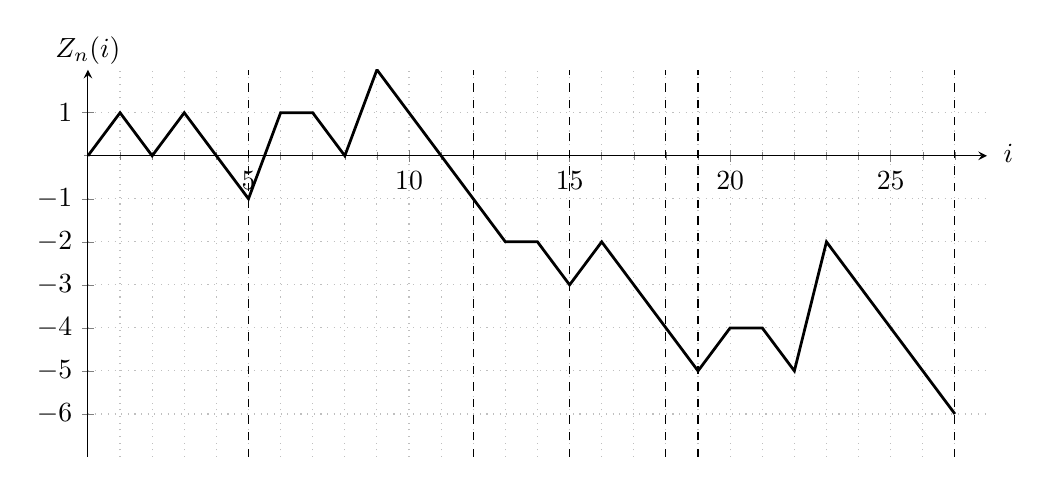
\begin{tikzpicture}

\begin{axis}[
axis x line=bottom,
axis y line=left,
grid = minor,
minor grid style={dotted},
xmin=0,
axis lines = middle,
xmax=28,
ymax = 2,
ymin  = -7,
xlabel={$i$},
x label style = {at={(axis description cs:1.04,0.785)},anchor=east},
ylabel={$Z_n(i)$},
y label style = {at={(axis description cs:0,1.11)},anchor=north},
xtick={5,10,15,20,25},
minor xtick = {1,...,27},
ytick={-6,...,1},
minor ytick={-6,...,1},
width = 13cm,
height = 6.5cm
]

\addplot [
line width=1.0pt
]
coordinates{
	(0,0) (1,1) (2,0) (3,1) (4,0) (5,-1)
	(6,1) (7,1) (8,0) (9,2) (10,1) (11,0) (12,-1) (13,-2) 
	(14,-2) (15,-3) 
	(16,-2) (17,-3) (18,-4) 
	(19,-5) 
	(20, -4) (21,-4) (22,-5) (23,-2) (24,-3) (25,-4) (26, -5) (27,-6)
};

\addplot [dashed] coordinates {(5, -7) (5, 2)};
\addplot [dashed] coordinates {(12, -7) (12, 2)};
\addplot [dashed] coordinates {(15, -7) (15, 2)};
\addplot [dashed] coordinates {(18, -7) (18, 2)};
\addplot [dashed] coordinates {(19, -7) (19, 2)};
\addplot [dashed] coordinates {(27, -7) (27, 2)};
\end{axis}

\end{tikzpicture} }
	
	\caption{A breadth-first walk on a random graph}
\end{figure} 
\fxnote{Fix random walk: Error around node 9!?}
\fxnote{Fix centering of figure captions}
\fxnote{Add lines indicating end of components in fig bf walk}
\fxnote{Add more vertex labels in original ordering?}


%%%%%%%%%%%%%%%%%%%%%%%%%%%%%%%%%%%%%%%%%%%%%%%%%%%%%%%%%%%%
% Equivalent definition
%%%%%%%%%%%%%%%%%%%%%%%%%%%%%%%%%%%%%%%%%%%%%%%%%%%%%%%%%%%%
We write
\begin{align}
\zeta(j) &:= |\Ci{1}| + \dots + |\Ci{j}|, \label{E: zeta}\\ 
\ZetaMinus{i} &:= \min \{ j \; | \; \zeta(j) \geq i \}, \label{E: zeta-1}
\end{align}
for the index of the last vertex in the $j$-th component (that's \eqref{E: zeta})
and \eqref{E: zeta-1}, the index of the component containing $v(i)$.
\fxnote{This sentence is a test for labeling of align-equs. Fix!}
Now we can provide a definition of the breadth-first walk equivalent to \eqref{E: def bf-walk z}:
\begin{equation}  \label{E: def bf-walk z*}
\begin{aligned}
z^*(0) &:= 0, \\
z^*(i) &:= |\Ni{i}| - \zeta^{-1}(i), \quad i=1, \dots , n.
\end{aligned}
\end{equation}

We verify the equivalence by induction.
We show that, for $i \geq 2$, increments of both functions are equal,
so
\begin{equation} \label{E: equality z z*}
\begin{aligned} 
&\hspace{35pt} z(i) - z(i-1) = z^*(i)  -z^*(i-1) \\
&\iff c(i) - 1 = |\Ni{i}| - \ZetaMinus{i} - |\Ni{i-1}| + \ZetaMinus{i-1} \\
&\iff |\Ni{i}| - |\Ni{i-1}| = c(i) + \ZetaMinus{i} - \ZetaMinus{i-1}
\end{aligned}
\end{equation}
\fxnote{This equation does not look nice. Delete 1./2. row? Delete iffs?}
\fxnote{This has to hold for i >= 1, or fix the indices.}

We divide the proof into two cases.
First, assume $v(i-1)$ is not the last vertex in it's component.
Then $v(i)$ belongs to the same component and
$\ZetaMinus{i} = \ZetaMinus{i-1}$.
Vertex $v(i)$ has already been assigned a new label at step $i-1$,
so $v(i) \in \Ni{i-1}$.
Going from $i-1$ to $i$,
$\Ni{*}$ increases by the number of new neighbours of $v(i)$
and decreases by $v(i)$ itself.
So
\begin{equation}
|\Ni{i}| - |\Ni{i-1}| = c(i) - 1,
\end{equation}
which proves the equivalence.

In the second case, if $v(i-1)$ is the last vertex of it's component,
then $\ZetaMinus{i} = \ZetaMinus{i-1} + 1$
and $|\Ni{i-1}| = 0$.
Equality \eqref{E: equality z z*} reduces to
$ |\Ni{i}| = c(i)$,
which holds since
$c(i) = |\Ni{i} \backslash \Ni{i-1}| = |\Ni{i}|$.

Since $|\Ni{i}| = 0$ only if $v(i)$ is the last vertex in its component,
\fxnote{Have we shown this? Maybe add a sentence.}
\fxnote{its or it's? Fix in whole document!}
\eqref{E: zeta} and \eqref{E: def bf-walk z*} imply
\begin{equation}
	z(\zeta (j)) = -j
\end{equation}
and 
\begin{equation}
	z(i) \geq -j \quad \text{for all} \enspace \zeta(j) < i < \zeta(j+1).
\end{equation}

So, for vertices in the $j$-th component,
the random walk takes values greater or equal to $-(j-1)$,
until the last vertex, for which $z$ reaches a new minimum at $-j$.
\fxnote{There are a lot of commas in this sentence.}
Knowing this we can reconstruct sizes and indices of components via
\begin{align}
\zeta(j) &= \min \{ i \; | \; z(i) = -j \}, \\
|\Ci{j}| &= \zeta(j) - \zeta(j-1), \\
\ZetaMinus{i} &= 1 - \min_{j \leq i-1}z(j).
\end{align}
\fxnote{Maybe add some more explanation on where these formulas come from.}




\section{The continuous breadth-first walk}
%%%%%%%%%%%%%%%%%%%%%%%%%%%%%%%%%%%%%%%%%%%%%%%%%%%%%%%%%%%%
% SECTION: The continuous breadth-first walk
%%%%%%%%%%%%%%%%%%%%%%%%%%%%%%%%%%%%%%%%%%%%%%%%%%%%%%%%%%%%


\section{Decompositions of $Z_n$}
%%%%%%%%%%%%%%%%%%%%%%%%%%%%%%%%%%%%%%%%%%%%%%%%%%%%%%%%%%%%
% SECTION: Decompositions of $Z_n$
%%%%%%%%%%%%%%%%%%%%%%%%%%%%%%%%%%%%%%%%%%%%%%%%%%%%%%%%%%%%
\fxfatal{Update title}
\fxnote{Add introductory text}

For ease of notation, we will drop the superscript $t$ from all random variables.


%%%%%%%%%%%%%%%%%%%%%%%%%%%%%%%%%%%%%%%%%%%%%%%%%%%%%%%%%%%%
% Lemma Decompositions 1: Statement
%%%%%%%%%%%%%%%%%%%%%%%%%%%%%%%%%%%%%%%%%%%%%%%%%%%%%%%%%%%%
\begin{lemma} \label{L: decomp Zn}
	The decomposition 
	\begin{equation} \label{E: decomp Zn}
	Z_n = M_n + A_n
	\end{equation}
	holds, where $M_n$ is a martingale and $A_n$ is defined by
	\begin{equation} \label{D: An}
	\An{t} = \int_{0}^{t} a_n(s)ds - t
	\end{equation}
	and
	\begin{equation} \label{D: an}
	a_n(s)ds = P(\text{A new edge appears in} \enspace [s, s+ds] \cond \Zn{u}, \enspace u \leq s).
	\end{equation}	
	\fxnote{Make text in P() not cursive?}
\end{lemma}
\begin{note} \label{N: decomp Zn}
	$A_n$ is a continuous process of bounded variation, so jumps of $M_n$ are the same as jumps of $Z_n$. Since $Z_n$ and $A_n$ are of bounded variation, $M_n$ is a cadlaq process of bounded variation.
	\fxnote{Proof that An is of bounded variation.}
	\fxnote{Proof that Mn is cadlaq.}	
\end{note}


%%%%%%%%%%%%%%%%%%%%%%%%%%%%%%%%%%%%%%%%%%%%%%%%%%%%%%%%%%%%
% Lemma Decompositions: Proof
%%%%%%%%%%%%%%%%%%%%%%%%%%%%%%%%%%%%%%%%%%%%%%%%%%%%%%%%%%%%
\begin{proof} \label{P: decomp Zn}
	We will prove that, for $A_n$ defined in \ref{D: An} and \ref{D: an},
	$Z_n - A_n$
	is a martingale by showing that
	\begin{equation} \label{E: Mn martingale}
	\Exp{ \Zn{t+u} - \An{t+u} \cond \F{t} } = \Zn{t} - \An{t} \quad \forall u \geq 0
	\end{equation}
	holds, where $\F{t}$ is the natural $\sigma$-algebra generated by $Z_n$, 
	$\F{t} = \sigma(\Zn{s}, s \leq t).$
	This is equivalent to 
	\begin{equation}
	\Exp{\Zn{t+u} - \Zn{t} \cond \F{t}} = \Exp{\An{t+u} - \An{t} \cond \F{t}}.
	\end{equation}
	
	We start with the left-hand side. 
	The difference between $Z_n$ at times $t$ and $t+u$ is the sum of all jumps that occurred in $[t, t+u]$ minus the constant downward drift $u$:
	\begin{align*}
	\Exp{\Zn{t+u} - \Zn{t} \cond \F{t}} 
	&= \Exp{\text{Number of jumps in} \enspace [t, t+u] \cond \F{t}} - u \\
	&= \Exp{\text{Number of new edges appearing in} \enspace [t, t+u] \cond \F{t}} - u,
	\end{align*}
	since every new edge corresponds to a jump of size $1$ in $Z_n$.
	
	Looking at the right-hand side, we define $\Esds$ as the event of a new edge appearing in the interval $[s,s+ds]$ and calculate
	\begin{align*}
	\Exp{\An{t+u} - \An{t} \cond \F{t}}
	&= \Exp{ \int_{0}^{t+u} a_n(s)ds - (t+u) - \int_{0}^{t} a_n(s)ds + t \cond \F{t} } \\
	&= \Exp{ \int_{t}^{t+u} a_n(s)ds \cond \F{t} } - u \\
	&= \int_{t}^{t+u} \Exp{a_n(s)ds \cond \F{t}} - u \\
	&= \int_{t}^{t+u} \Exp{ P(\Esds \cond \F{s}) \cond \F{t} } - u\\
	&= \int_{t}^{t+u} P( \Esds \cond \F{t} ) - u
	\quad \text{since} \enspace \F{s} \subseteq \F{t} \enspace \forall s \in [t,t+u] \\
	&= \Exp{\text{Number of new edges appearing in} \enspace [t, t+u] \cond \F{t}} - u.
	\end{align*}
	\fxnote{Fs in Ft or Ft in Fs? Use "tower property".}
	\fxnote{Explain "Number of new edges"="int P" more detailed.}
	
	This proves $M_n$ to be a martingale. 	
\end{proof}


%%%%%%%%%%%%%%%%%%%%%%%%%%%%%%%%%%%%%%%%%%%%%%%%%%%%%%%%%%%%
% Lemma Decompositions 1: Statement
%%%%%%%%%%%%%%%%%%%%%%%%%%%%%%%%%%%%%%%%%%%%%%%%%%%%%%%%%%%%
\begin{lemma} \label{L: decomp Mn}
	The decomposition
	\begin{equation} \label{E: decomp Mn}
	M_n^2 = Q_n + B_n
	\end{equation}
	holds where $Q_n$ is a martingale and $B_n$ is defined by 
	\begin{equation} \label{D: An}
	\Bn{t} = \int_{0}^{t} a_n(s)ds = A_n(t) + t
	\end{equation}
	with $a_n$ defined in \ref{D: an}.
\end{lemma}
\begin{note} \label{N: decomp Mn}
	$B_n$ is a continuous process.
\end{note}


%%%%%%%%%%%%%%%%%%%%%%%%%%%%%%%%%%%%%%%%%%%%%%%%%%%%%%%%%%%%
% Lemma Decompositions 1: Proof
%%%%%%%%%%%%%%%%%%%%%%%%%%%%%%%%%%%%%%%%%%%%%%%%%%%%%%%%%%%%
\begin{proof} \label{P: decomp Mn}
	We will prove that
	$M_n^2 - B_n$
	is a martingale.
	Since $M_n$ is a right-continuous process of bounded variation, its quadratic variation
	\begin{equation*} \label{D: quadratic variation}
	[M]_t := \limsup \sum (M_{t_i} - M_{t_{i-1}})^2
	\end{equation*}
	\fxnote{Add definition of quadratic variation.}
	is
	\begin{equation} \label{E: quadratic variation Mn}
	\Mnq{t} = \sum_{0 \leq s \leq t} (\Delta \Mn{s})^2,
	\end{equation}
	where
	$\Delta \Mn{s} := \Mn{s} - \Mn{s-}$ 
	can take one of two values: $1$ if there is a jump of $1$ at time $s$, 0 otherwise.
	\fxnote{Other word for "take".}
	We refer to [EK] to see that
	$M_n^2 - [M_n]$
	is a martingale.
	\fxnote{Add reference from [EK]}
	\fxnote{Nicer sentence.}
	Thus
	\begin{equation}
	M_n^2 - B_n = (\underbrace{M_n^2 - [M_n]}_{\text{martingale}}) + ([M_n] - B_n)
	\end{equation}
	and to prove \ref{decomp Mn} it suffices to show that
	$[M_n] - B_n$
	is a martingale.
	Using the fact that the jumps of $M_n$ are the jumps of $Z_n$ and
	$\Delta Z_n \in \lbrace0,1 \rbrace$
	we calculate
	\begin{align*}
	\Mnq{t} - \Bn{t}
	&= \sum_{0 \leq s \leq t} (\Delta \Mn{s})^2 - \Bn{t} \\
	&= \sum_{0 \leq s \leq t} (\Delta \Zn{s})^2 - \Bn{t} \\
	&= \sum_{0 \leq s \leq t} \Delta \Zn{s} - \Bn{t} \\
	&= \text{Number of jumps of} \enspace Z_n \enspace \text{in} \enspace [0,t] - \Bn{t} \\
	&= (\text{Number of jumps of} \enspace Z_n \enspace \text{in} \enspace [0,t] - t) - \An{t} \\
	&= \Zn{t} - \An{t}
	\end{align*}
	which is a martingale from Lemma \ref{L: decomp Zn}.
	
\end{proof}


%%%%%%%%%%%%%%%%%%%%%%%%%%%%%%%%%%%%%%%%%%%%%%%%%%%%%%%%%%%%
% Lemma Formula An: Statement
%%%%%%%%%%%%%%%%%%%%%%%%%%%%%%%%%%%%%%%%%%%%%%%%%%%%%%%%%%%%
\begin{lemma} \label{L: formula an}
	For $a_n$ as in the Lemmas above,
	\begin{equation}
		\an{s} = (n - s - \Zetan{\ceil{s}} - \Zn{s}) \ps .
	\end{equation}
	\fxnote{Update/change Zeta-symbol if needed.}
	\fxnote{Add explanation of Zeta if needed.}
\end{lemma}


%%%%%%%%%%%%%%%%%%%%%%%%%%%%%%%%%%%%%%%%%%%%%%%%%%%%%%%%%%%%
% Lemma Formula An: Proof
%%%%%%%%%%%%%%%%%%%%%%%%%%%%%%%%%%%%%%%%%%%%%%%%%%%%%%%%%%%%
\begin{proof} \label{P: formula an}
	proof.
	\fxnote{Add proof.}
\end{proof}


\section{Asymptotics}
%%%%%%%%%%%%%%%%%%%%%%%%%%%%%%%%%%%%%%%%%%%%%%%%%%%%%%%%%%%%
% SECTION: Asymptotics
%%%%%%%%%%%%%%%%%%%%%%%%%%%%%%%%%%%%%%%%%%%%%%%%%%%%%%%%%%%%
\fxfatal{Update title.}

We will now prove some limit properties of the processes $A_n$, $B_n$ and $M_n$ with the goal of using the functional central limit theorem for martingales.
\fxnote{Update text.}


%%%%%%%%%%%%%%%%%%%%%%%%%%%%%%%%%%%%%%%%%%%%%%%%%%%%%%%%%%%%
% Lemma Limit An: Statement
%%%%%%%%%%%%%%%%%%%%%%%%%%%%%%%%%%%%%%%%%%%%%%%%%%%%%%%%%%%%
\begin{lemma} \label{L: limit An}
	For $A_n$ defined as in the previous Lemmas and a fix $s_0 \geq 0$,
	\begin{equation} \label{E: limit An}
	\n{-1}{3} \supns \left| \An{s} + n^{-1}\frac{s^2}{2} - \n{-1}{3}st \right| \longrightarrow_p 0,
	\end{equation}
	where $t$ is the fixed probability parameter of the random graph.
	\fxnote{Change/remove explanation of t: "probability parameter"}	
\end{lemma}


%%%%%%%%%%%%%%%%%%%%%%%%%%%%%%%%%%%%%%%%%%%%%%%%%%%%%%%%%%%%
% Lemma Limit An: Proof
%%%%%%%%%%%%%%%%%%%%%%%%%%%%%%%%%%%%%%%%%%%%%%%%%%%%%%%%%%%%
\begin{proof} \label{P: limit An}
	We define $\amn{s}$ as
	\begin{equation}
		\amn{s} := (n - s - \Zetan{\ceil{s}} - \Zn{s}) p(n),
	\end{equation}
	which is $a_n$ without the denominator.
	\fxnote{Change "without the denominator"}
	First, we show that $\an{s}$ and $\amn{s}$ converge uniformly in $s$.
	\begin{equation}
	proof
	\end{equation}
	\fxnote{Add proof of uniform convergence.}
	Now we use the definition of $p(n)$ to expand
	\begin{align*}
	\amn{s} - 1 
	&= \left( n - s - \Zetan{\ceil{s}} - \Zn{s} \right) \left( n^{-1} + t\n{-4}{3} \right) - 1 \\
	&= 1 + t\n{-1}{3} - sn^{-1} - st\n{-4}{3} \\
	&\quad - \left( \Zetan{\ceil{s}} + \Zn{s} \right) \left( n^{-1} + t\n{-4}{3} \right) -1 .
	\end{align*}
	Thus
	\begin{equation} \label{E: (27)} 
	\begin{aligned}
	\left| \amn{s} - 1 + \frac{s}{n} - \frac{t}{\n{1}{3}} + \frac{st}{\n{4}{3}} \right|
	&= \left| \frac{\Zetan{\ceil{s}} + \Zn{s}}{n} \left( 1 + \frac{t}{\n{1}{3}} \right) \right| \\
	&\leq 2 \left| \frac{\Zetan{\ceil{s}} + \Zn{s}}{n} \right| \\
	&\leq 2 \frac{\Zetan{\ceil{s}} + |\Zn{s}|}{n} ,  
	\end{aligned}
	\end{equation}
	for $\n{1}{3} \geq |t|$. Note that $\Zetan{\ceil{s}} \geq 0$ for all $s \geq 0$.
	Integrating the inner part of the left-hand side over $s$ yields
	\fxnote{Make clear: We integrate the inner part of the LHS from 0 to s.}
	\begin{align*}
	\int_{0}^{s} \amn{u} - 1 + \frac{u}{n} - \frac{t}{\n{1}{3}} + \frac{ut}{\n{4}{3}} du
	&= \int_{0}^{s} \amn{u} - 1 du + \frac{s^2}{2n} - \frac{st}{\n{1}{3}} + \frac{s^2t}{2\n{4}{3}} \\
	&\xrightarrow{n \rightarrow \infty} \An{s} + \frac{s^2}{2n} - \frac{st}{\n{1}{3}} + \frac{s^2t}{2\n{4}{3}},
	\end{align*}
	Using \ref{L: zeta(i)}, the following inequalities hold for sufficiently large $n$:
	\fxnote{Add reference to lemma.}
    \begin{align*}
    \left| \An{s} + \frac{s^2}{2n} - \frac{st}{\n{1}{3}}  + \frac{s^2t}{2\n{4}{3}}  \right| 
    &= \left| \int_{0}^{s} \amn{u} - 1 + \frac{u}{n} - \frac{t}{\n{1}{3}} + \frac{ut}{\n{4}{3}} du \right| \\
    &\leq \int_{0}^{s} \left|\amn{u} - 1 + \frac{u}{n} - \frac{t}{\n{1}{3}} + \frac{ut}{\n{4}{3}} \right| du \\
    &\leq \int_{0}^{s} 2 \frac{\Zetan{\ceil{u}} + |\Zn{u}|}{n} du \\
    &= \frac{2}{n}  \int_{0}^{s} 1-\min_{w \leq \ceil{u}-1} \Zn{w}  + |\Zn{u}| du \\
    &= \frac{2}{n}  \int_{0}^{s} |\Zn{u}| - \min_{w \leq \ceil{u}-1} \Zn{w} du + \BigO{\frac{s}{n}} \\
    &\leq \frac{4}{n} \max_{u \leq s} |\Zn{u}| + \BigO{\frac{s}{n}},
    \end{align*}
    the last inequality since $\ceil{u}-1 \leq s$ for $u\leq s$ and thus $|\min_{w \leq \ceil{u}-1}\Zn{w}| \leq \max_{u \leq s}|\Zn{u}|$.
    
    We define $A^*_n(s) := \An{s} + \frac{s^2}{2n} - \frac{st}{\n{1}{3}}$ and consider the difference
    \begin{align*}
    &\n{-1}{3}\supns | A^*_n{s} + \frac{s^2t}{2\n{4}{3}}  | - \n{-1}{3}\supns | A^*_n{s} | \\
    &\leq \n{-1}{3} \left( \supns | A^*_n{s} | + \supns |\frac{s^2t}{2\n{4}{3}}|  - \n{-1}{3}\supns | A^*_n{s} | \right) \\
    &= \n{-1}{3} \supns |\frac{s^2t}{2\n{4}{3}}| \\
    &= \n{-1}{3} \frac{s_0^2t}{2} \\
    &\xrightarrow{n \rightarrow \infty} 0,
    \end{align*}
    to see that proving
    \begin{align*}
    \n{-1}{3} \supns \frac{4}{n} \max_{u \leq s} |\Zn{u}| 
    &\leq 4 s_0 \n{-2}{3} \supns |\Zn{s}| \\
    &\longrightarrow_p 0 
    \end{align*}
    will suffice to prove \ref{E: limit An}.
    For that, we will prove the stronger result 
    \begin{equation}
    n^{-2/3} \sup_{s\leq n^{-1/3} s_0} |Z_n(s)| 
    \enspace \text{is stochastically bounded as} \enspace n \rightarrow \infty ,
    \end{equation} 
    i.e. for any 
    $ \epsilon > 0 $ 
    there is a
    $ K > 0 $
    such that for $n$ sufficiently big 
    \begin{equation} \label{E: stoch bounded}
    P\left( n^{-1/3} \sup_{s\leq n^{2/3} s_0} |Z_n(s)| > K \right) < \epsilon. 
    \end{equation}
    
    Let $T^*_n$ be the first time $\n{-1}{3}|Z_n(s)|$ surpasses $K$ and  
    $T_n := T^*_n$ 
    if 
    $T^*_n \leq \n{2}{3}s_0$
    or else
    $\n{2}{3}s_0:$
    \begin{align*}
    T_n &:= \min \lbrace T^*_n, \n{2}{3}s_0 \rbrace , \\
    T^*_n &:= \min \lbrace s: |Z_n(s)| > K \n{1}{3} \rbrace .
    \end{align*}
    \fxnote{Define Tn, T*n nicer.}
    Thus 
    \begin{equation} \label{E: stoch bounded 2}
    \begin{aligned}
    P( \sup_{s\leq n^{2/3} s_0} |Z_n(s)| > K \n{1}{3} ) &= P ( |Z_n(T_n)| > K\n{1}{3} ) \\
    &\leq \frac{\Exp{|Z_n(T_n)}}{K}
    \end{aligned} 
    \end{equation}
    by Markov's inequality.
    To analyse $\Exp{|Z_n(T_n)|}$ we will use the previously established decompositions
    $Z_n = M_n + A_n$ and $M^2_n = Q_n + B_n$, 
    starting with the latter:
    
    Since $Q_n$ is a martingale, by the optional sampling theorem
    $\Exp{Q_n(\tau)} = 0$ 
    for all stopping times $\tau$.
    \begin{align*}
    \Exp{M^2_n(T_n)} &= \Exp{B_n(T_n)} \\
    &= \Exp{ \int_{0}^{T_n} a_n(s)ds } \\
    &= \int_{0}^{T_n} \Exp{a_n(s)} ds.
    \end{align*} 
    By definition
    \begin{align*}
    a_n(s) &= (n - \nu_n(s)) \frac{p(n)}{1 - (s - \floor{s})p(n)} \\
    &\leq \frac{n p(n)}{1 - (s - \floor{s})p(n)}
    \end{align*}
    which is a deterministic function in $s$. So
    $ \Exp{a_n(s)} \leq \frac{n p(n)}{1 - (s - \floor{s})p(n)} $
    and
    \begin{align*}
    \int_{0}^{T_n} \Exp{a_n(s)} ds &\leq  \int_{0}^{T_n }\frac{n p(n)}{1 - (s - \floor{s})p(n)} \\
    &\leq \int_{0}^{\n{2}{3}s_0}\frac{n p(n)}{1 - (s - \floor{s})p(n)} \\
    &\leq 2\n{2}{3}s_0,
    \end{align*}
    where the last inequality holds for $n$ sufficiently large, since 
    $\frac{n p(n)}{1 - (s - \floor{s})p(n)} \rightarrow 1$
    as $n \rightarrow \infty$.
    We conclude
    \begin{equation} \label{E: exp Mn}
    \Exp{M_n(T_n)} \leq (2s_0)^{1/2}\n{1}{3}
    \end{equation}
    and move to $A_n$.
    
    Using \ref{E: (27)} and \ref{L: zeta(i)} we obtain
    \begin{align*}
    \Exp{|\An{T_n}|} &\leq \Exp{\int_{0}^{T_n} |\an{s}-1|ds} \\
    &\leq \Exp{\int_{0}^{\n{2}{3}s_0} |\an{s}-1|ds} \\
    &\leq \Exp{
    	\int_{0}^{T_n} | \an{s} + \amn{s} - \amn{s} + \frac{s}{n} - \frac{t}{\n{1}{3}} + \frac{st}{\n{4}{3}
    	} \\
    &\qquad \qquad - \frac{s}{n} + \frac{t}{\n{1}{3}} - \frac{st}{\n{4}{3}} | ds} \\
    &\leq \Exp{
    	\int_{0}^{T_n} |\an{s} - \amn{s}|ds \\
    	&\qquad + \int_{0}^{T_n} |\frac{s}{n} - \frac{t}{\n{1}{3}} + \frac{st}{\n{4}{3}}| ds \\
    	&\qquad + \int_{0}^{T_n} |\amn{s} - 1 + \frac{s}{n} - \frac{t}{\n{1}{3}} + \frac{st}{\n{4}{3}}|
    } \\
    &\leq \n{2}{3}s_0 \BigO{\frac{1}{n}} + \n{2}{3}s_0 \BigO{\frac{|t|}{\n{1}{3}}} \\
    &\qquad +  \n{2}{3}s_0 \left( \frac{4s}{n} \max_{u \leq T_n}|\Zn{u}| + \BigO{\frac{T_n}{n}}\right) \\
    &\leq 4 s_0 K + s_0|t|\BigO{\n{1}{3}} + s_0^2\BigO{\n{1}{3}} + s_0\BigO{\frac{1}{\n{1}{3}}},
    \end{align*}
    \fxnote{Fix BigO-Notation (Sapozhnikov?)}
    since, by definition of $T_n$, $|\Zn{T_n}| < K\n{1}{3}.$
    
    This and \ref{E: exp Mn} lead to a bound for large $n$:
    \begin{equation} \label{E: bound Zn}
    \Exp{|\Zn{T_n}|} \leq \alpha\n{1}{3} + 4s_0K,
    \end{equation}
    where $\alpha = \alpha(s_0,t)$ but not dependent on $n$ and $K$. 
    Substituting $\Exp{|\Zn{T_n}|}$ in \ref{E: stoch bounded 2} we arrive at
    \begin{equation}
    P( \sup_{s\leq n^{2/3} s_0} |Z_n(s)| > K \n{1}{3} ) \leq \frac{\alpha}{K} + \frac{4s_0}{\n{1}{3}}
    \end{equation}
    which proves \ref{E: stoch bounded}.
\end{proof}


%%%%%%%%%%%%%%%%%%%%%%%%%%%%%%%%%%%%%%%%%%%%%%%%%%%%%%%%%%%%
% Lemma Limit Bn: Statement
%%%%%%%%%%%%%%%%%%%%%%%%%%%%%%%%%%%%%%%%%%%%%%%%%%%%%%%%%%%%
\begin{lemma} \label{L: limit Bn}
	For $B_n$ defined as in the previous Lemmas and a fix $s_0 \geq 0$,
	\begin{equation} \label{E: limit Bn}
	\n{-2}{3} \Bn{\n{2}{3}s_0} \longrightarrow_p s_0,
	\end{equation}
	as $n \longrightarrow \infty$.
\end{lemma}


%%%%%%%%%%%%%%%%%%%%%%%%%%%%%%%%%%%%%%%%%%%%%%%%%%%%%%%%%%%%
% Lemma Limit Bn: Proof
%%%%%%%%%%%%%%%%%%%%%%%%%%%%%%%%%%%%%%%%%%%%%%%%%%%%%%%%%%%%
\begin{proof} \label{P: limit Bn}
	From its definition in Lemma \ref{L: decomp Mn}, $\Bn{s} = \An{s} + s$, which allows us to rewrite \ref{E: limit Bn} as
	\begin{equation} \label{E: limit Bn An}
	\n{-2}{3} \An{\n{-2}{3}s_0} \rightarrow_p 0.
	\end{equation}
	We will show that
	\begin{equation} \label{E: limit Bn An + c}
	\n{-1}{3} \An{\n{-2}{3}s_0} + \frac{1}{2}s_0^2 - s_0t \longrightarrow_p 0,
	\end{equation}
	where again $t$ denotes the probability parameter. 
	\fxnote{Change "probability parameter"}
	This implies
	\begin{equation*}
	\n{-1}{3} \left( \n{-1}{3} \An{\n{-2}{3}s_0} + \frac{1}{2}s_0^2 - s_0t \right) \longrightarrow_p 0
	\end{equation*}
	which, since $\frac{1}{2}s_0^2 - s_0t$ is a constant in $n$, proves \ref{E: limit Bn An}.
	
	Let the function $\phi$ be defined by $\phi(s) = \frac{1}{2}\n{-4}{3}s^2 - \n{-2}{3}st$.	
	Now $\phi(\n{2}{3}s_0) = \frac{1}{2}s_0^2 - s_0t$ and
	\begin{align*}
	\left| \n{-1}{3} \An{\n{-2}{3}s_0} + \frac{1}{2}s_0^2 - s_0t \right| 
	&= \left| \n{-1}{3} \An{\n{-2}{3}s_0} + \phi(\n{2}{3}s_0) \right| \\
	&\leq \supns \left| \n{-1}{3} \An{s} + \phi(s) \right| \\
	&= \n{-1}{3} \supns \left| \An{s} + n^{-1}\frac{s^2}{2} - \n{-1}{3}st \right| \\
	&\longrightarrow_p 0,
	\end{align*}
	as $n \rightarrow \infty$ from Lemma \ref{L: limit An}. This gives \ref{E: limit Bn An + c} and completes the proof.
\end{proof}


%%%%%%%%%%%%%%%%%%%%%%%%%%%%%%%%%%%%%%%%%%%%%%%%%%%%%%%%%%%%
% Lemma Limit Mn: Statement and Proof
%%%%%%%%%%%%%%%%%%%%%%%%%%%%%%%%%%%%%%%%%%%%%%%%%%%%%%%%%%%%
\begin{lemma} \label{L: limit Mn}
	For $M_n$ defined as in the previous Lemmas and a fix $s_0 \geq 0$,
	\begin{equation} \label{E: limit Mn}
	\n{-2}{3} \Exp{\supns |\Mn{s} - \Mn{s-}|^2} \longrightarrow s_0,
	\end{equation}
	as $n\longrightarrow \infty$.
\end{lemma}

\begin{proof} \label{P: limit Mn}
	As previously discussed in the proof of Lemma \ref{L: decomp Mn}, the jumps of $M_n$ are exactly the jumps of $Z_n$ and thus have size $1$. The lemma follows immediately.
\end{proof}


\section{The central limit theorem for martingales}
%%%%%%%%%%%%%%%%%%%%%%%%%%%%%%%%%%%%%%%%%%%%%%%%%%%%%%%%%%%%
% SECTION: The central limit theorem for martingales
%%%%%%%%%%%%%%%%%%%%%%%%%%%%%%%%%%%%%%%%%%%%%%%%%%%%%%%%%%%%
\fxfatal{Update title}


%%%%%%%%%%%%%%%%%%%%%%%%%%%%%%%%%%%%%%%%%%%%%%%%%%%%%%%%%%%%
% Definitions: Rescaled process
%%%%%%%%%%%%%%%%%%%%%%%%%%%%%%%%%%%%%%%%%%%%%%%%%%%%%%%%%%%%
We now define the rescaled processes 
$\bar{M}_n(s) = \n{-1}{3}\Mn{\n{2}{3}s}$, 
$\bar{A}_n(s) = \n{-1}{3}\An{\n{2}{3}s}$, 
$\bar{Q}_n(s) = \n{-2}{3}Q_n(\n{2}{3}s)$ and 
$\bar{B}_n(s) = \n{-2}{3}B_n(\n{2}{3}s)$ to fit the previously rescaled process 
$\bar{Z}_n$ from \ref{D: rescaled Zn}, such that
\begin{align*}
\Zbar{s} &= \Mbar{s} + \Abar{s} \\
\bar{M}_n^2(s) &= \bar{Q}_n(s) + \Bbar{s}.
\end{align*}
\fxnote{Definition of rescaled processes tidier.}

Rescaling Lemmas \ref{L: limit An}, \ref{L: limit Bn} and \ref{L: limit Mn} gives us
\begin{equation} \label{E: limit An rescaled}
\sup_{s \leq s_0} |\Abar{s} - \rho (s)| \longrightarrow_p 0,
\end{equation}
where $\rho (s) = st - \frac{1}{2}s^2$,
\begin{equation} \label{E: limit Bn rescaled}
\Bbar{s_0} \longrightarrow_p s_0,
\end{equation}
and
\begin{equation} \label{E: limit Mn rescaled}
\Exp{\sup_{s \leq s_0} | \Mbar{s} - \Mbar{s-} |^2 } \longrightarrow 0.
\end{equation}
We now use the central limit theorem for martingales to prove te convergence of $\bar{M}_n$ to a Brownian motion.
We state the theorem here, without proof, as it appears in \cite[p. 339 f.]{N.Ethier1986},
omitting one of two equivalent conditions and all references to higher dimensional processes to focus on the one-dimensional case we will need for our proof.


%%%%%%%%%%%%%%%%%%%%%%%%%%%%%%%%%%%%%%%%%%%%%%%%%%%%%%%%%%%%
% Central limit theorem for martingales: Statement
%%%%%%%%%%%%%%%%%%%%%%%%%%%%%%%%%%%%%%%%%%%%%%%%%%%%%%%%%%%%
\begin{theorem}[Central limit theorem for martingales] \label{T: functional CLT martingales}
	Let $\{\Fn{t}\}$ be a filtration and $M_n$ a $\{\Fn{t}\}$-local martingale with sample paths in $D_{\Real}[0,\infty)$ and $\Mn{0}=0$.
	Let $B_n$ be a process with sample paths in $D_{\Real}[0,\infty)$, increasing in $t$, such that $M_n^2 - B_n$ is an $\{\Fn{t}\}$-local martingale.
	
	Let the following conditions hold:
	For each $T>0$,
	\begin{equation} \label{E: cond1 CLT}
	\lim_{n->\infty} \ExpBig{
	\sup_{t \leq T} | \Bn{t} - \Bn{t-}|
    } = 0,
	\end{equation}
	\begin{equation} \label{E: cond2 CLT}
	\lim_{n->\infty} \ExpBig{
		\sup_{t \leq T} | \Mn{t} - \Mn{t-}|^2
	} = 0,
	\end{equation}
	and with $c(t)$ a continuous, increasing function on $[0, \infty)$, $c(0) = 0$, let
	\begin{equation} \label{E: cond3 CLT}
	\Bn{t} \longrightarrow_p c(t).
	\end{equation}
	Then $M_n \longrightarrow_d X$ where $x$ is a process with sample paths in $C_{\Real}[0,\infty)$ and independent Gaussian increments.
\end{theorem}


%%%%%%%%%%%%%%%%%%%%%%%%%%%%%%%%%%%%%%%%%%%%%%%%%%%%%%%%%%%%
% Theorem Convergence Z_n: Proof
%%%%%%%%%%%%%%%%%%%%%%%%%%%%%%%%%%%%%%%%%%%%%%%%%%%%%%%%%%%%
We are now ready to prove Theorem \ref{T: convergence Zn}.

\begin{proof}[Proof of Theorem \ref{T: convergence Zn}]
	Let again $\{\Fn{t}\}$ be the filtration generated by $Z_n$, 
	$\Fn{t} = \sigma \{ \Zn{s}, s \leq t \}$.
	The rescaling above does not alter martingale properties of the resulting processes,
	so $\bar{M}_n$ and $\bar{Q}_n = \bar{M}_n^2 - \bar{B}_n$ are still martingales in $\{\Fn{t}\}$.
	\fxnote{Martingales for/in?}
	\fxnote{Martingale = F-local martingale?}
	We apply Theorem \ref{T: functional CLT martingales} to $\bar{M}_n$ and $\bar{B}_n$.
	The continuity of $\bar{B}_n$ satisfies condition \ref{E: cond1 CLT}, 
	condition \ref{E: cond2 CLT} holds from \ref{E: limit Mn rescaled}
	and \ref{E: limit Bn rescaled} gives condition \ref{E: cond3 CLT}, with $c(t) := t$.
	
	Thus $\Mbar{s} \rightarrow_d W(s)$, the standard Brownian motion, and by using \ref{E: limit An rescaled} we obtain
	\begin{equation*}
	\Zbar{s} = \Mbar{s} + \Abar{s} \rightarrow_d W(s) + \rho (s) = W^t(s).
	\end{equation*}
			
\end{proof}

